\documentclass{article}
\usepackage{cmap}
\usepackage[utf8]{inputenc}
\usepackage[english,ukrainian]{babel}
\usepackage{graphicx}
\usepackage{geometry}
\usepackage{listings}
\usepackage{float}
\usepackage{amsmath}
\usepackage{bm}
\geometry{
	a4paper,
	left=20mm,
	right=20mm,
	top=20mm,
	bottom=20mm
}
\lstset{
	language=c,
	tabsize=4,
	keepspaces,
	showstringspaces=false,
}
\graphicspath{ {./pictures} }
\setlength{\parindent}{4em}

\newcommand\subject{Операційні системи}
\newcommand\lecturer{старший викладач кафедри ПЗ\\Грицай О.Д.}
\newcommand\teacher{старший викладач кафедри ПЗ\\Грицай О.Д.}
\newcommand\mygroup{ПЗ-22}
\newcommand\lab{1}
\newcommand\theme{Ознайомлення та керування процесами в операційних системах для
	персонального комп’ютера. Windows}
\newcommand\purpose{Ознайомитися з процесами та потоками в операційній системі	Windows. Навчитися працювати із системними утилітами, що дають	можливість отримувати інформацію про процеси, потоки, використовувану ними пам'ять, та іншу необхідну інформацію}

\begin{document}
\begin{normalsize}
	\begin{titlepage}
		\thispagestyle{empty}
		\begin{center}
			\textbf{МІНІСТЕРСТВО ОСВІТИ І НАУКИ УКРАЇНИ\\
				НАЦІОНАЛЬНИЙ УНІВЕРСИТЕТ "ЛЬВІВСЬКА ПОЛІТЕХНІКА"}
		\end{center}
		\begin{flushright}
			Інститут \textbf{КНІТ}\\
			Кафедра \textbf{ПЗ}
		\end{flushright}
		\vspace{200pt}
		\begin{center}
			\textbf{ЗВІТ}\\
			\vspace{10pt}
			До лабораторної роботи № \lab\\
			\textbf{На тему}: “\textit{\theme}”\\
			\textbf{З дисципліни}: “\subject”
		\end{center}
		\vspace{112pt}
		\begin{flushright}
			
			\textbf{Лектор}:\\
			\lecturer\\
			\vspace{28pt}
			\textbf{Виконав}:\\
			
			студент групи \mygroup\\
			Коваленко Д.М.\\
			\vspace{28pt}
			\textbf{Прийняла}:\\
			
			\teacher\\
			
			\vspace{28pt}
			«\rule{1cm}{0.15mm}» \rule{1.5cm}{0.15mm} 2022 р.\\
			$\sum$ = \rule{1cm}{0.15mm}……………\\
			
		\end{flushright}
		\vspace{\fill}
		\begin{center}
			\textbf{Львів — 2022}
		\end{center}
	\end{titlepage}
		
	\begin{description}
		\item[Тема.] \theme.
		\item[Мета.] \purpose.
	\end{description}

	\section*{Лабораторне завдання}
	\begin{enumerate}
		\item За допомогою утиліти «Диспетчер задач» та Process Explorer отримати
		повну інформацію про процеси: ідентифікатор процесу, завантаження ЦП
		(центрального процесора), час ЦП, базовий пріоритет, стан процесу,
		пам'ять-використання, пам'ять-зміни, пам'ять-максимум, помилок сторінки,
		об’єкти USER, код сеансу, об’єм віртуальної пам’яті, лічильник дескрипторів,
		лічильник потоків.
		\item За допомогою утиліти Process Explorer отримати додаткову інформацію
		про процеси та їхні потоки.
		\item Використовуючи «Диспетчер задач» та Process Explorer змінити
		пріоритет будь-якого процесу, від низького до «реального часу»; задати
		відповідність виконання процесів на окремих ядрах центрального процесора;
		виконати завершення процесу.
		\item Використовуючи Process Explorer призупинити процес і відновити його
		роботу.
		\item Скомпілювати файл main.cpp представлений нижче і запустити
		виконуваний файл на різній кількості активних процесорів (ядер). Знайти для
		даної програми величини  A, S, p при різних вхідних значеннях величини n.
		\item Дослідити вплив зміни відповідності ядру на швидкодію процесу.
		Виконати завдання згідно варіанту, що відповідає порядковому номеру у
		списку підгрупи.
		\begin{center}
			2) Стискання файлів
		\end{center}
		\item Результати лабораторної роботи оформити у звіт, у висновку надати
		порівняння моніторингу процесів у різних системах різними утилітами.
	\end{enumerate}

	\section*{Хід роботи}
	\subsection*{1. Отримати повну інформацію про процеси.}
	У вікні "Select Columns" виберу необхідні поля: ідентифікатор процесу, завантаження ЦП (центрального процесора), час ЦП, базовий пріоритет, стан процесу, пам'ять-використання, пам'ять-зміни, пам'ять-максимум, помилок сторінки, об’єкти USER, код сеансу, об’єм віртуальної пам’яті, лічильник дескрипторів, лічильник потоків.
	\begin{figure*}[h]
		\centering
		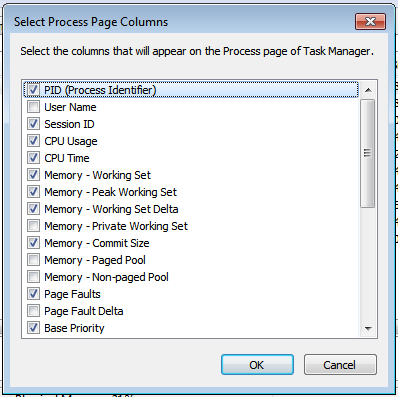
\includegraphics[scale=0.42]{1}~~~~~
		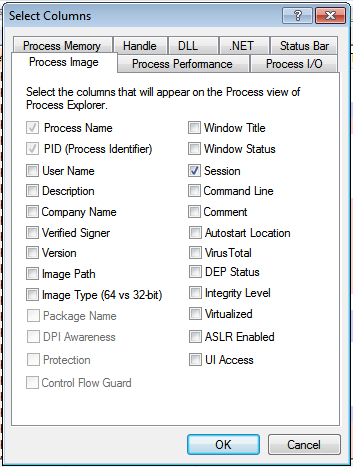
\includegraphics[scale=0.42]{2}
	\end{figure*}

	\subsection*{2. Отримати додаткову інформацію про процеси та їх потоки.}
	\begin{center}
		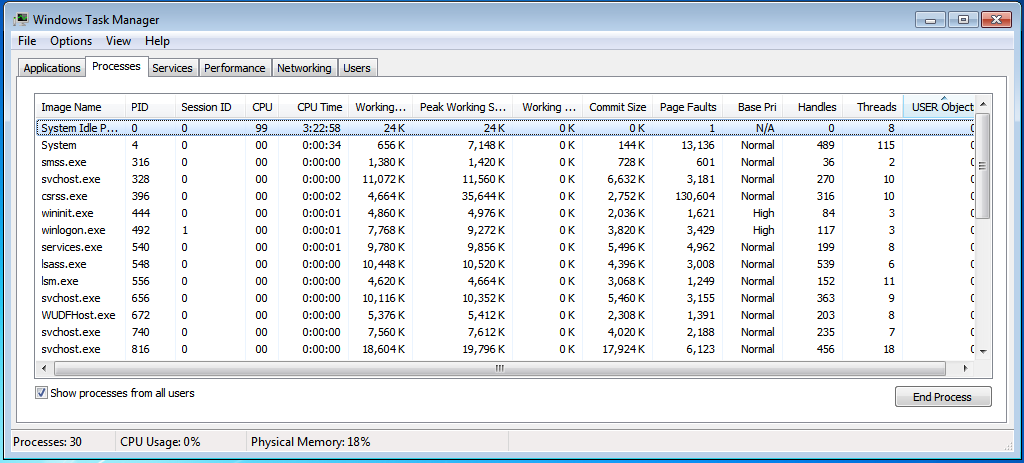
\includegraphics[scale=0.49]{usual1}
	\end{center}
	
	\begin{center}
		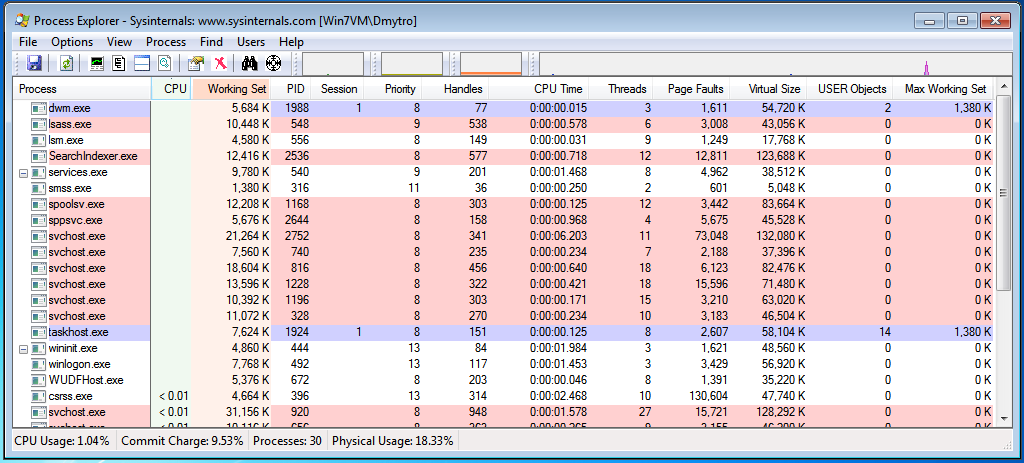
\includegraphics[scale=0.49]{usual2}
	\end{center}
	
	\subsection*{3.1 Змінити пріоритет будь-якого процесу.}
	\begin{center}
		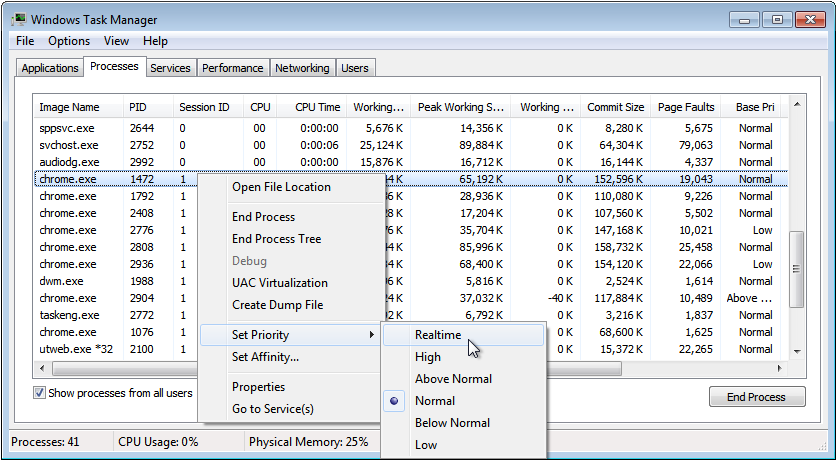
\includegraphics[scale=0.6]{priority1}
	\end{center}
	
	\begin{center}
		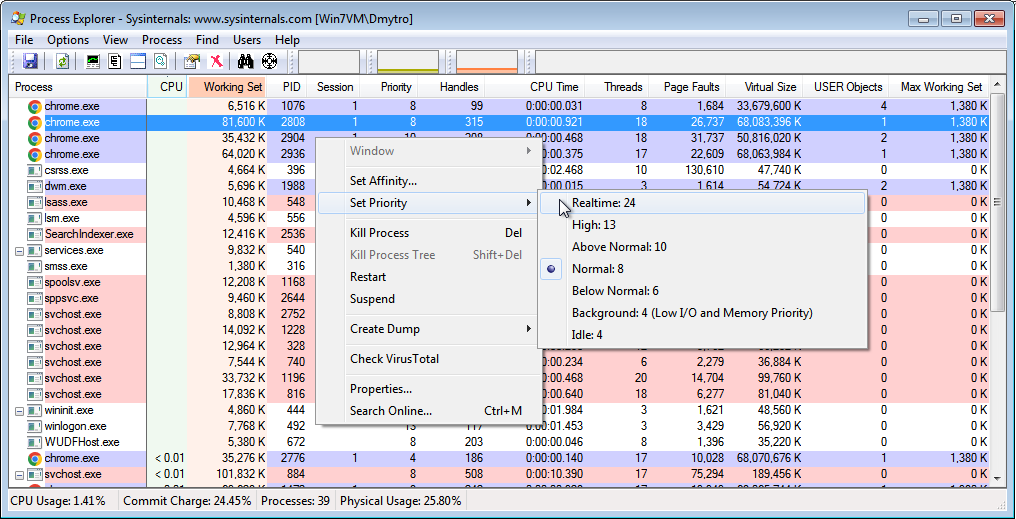
\includegraphics[scale=0.49]{priority2}
	\end{center}

	\subsection*{3.2 Задати відповідність виконання процесу на окремих ядрах ЦП.}
	\begin{center}
		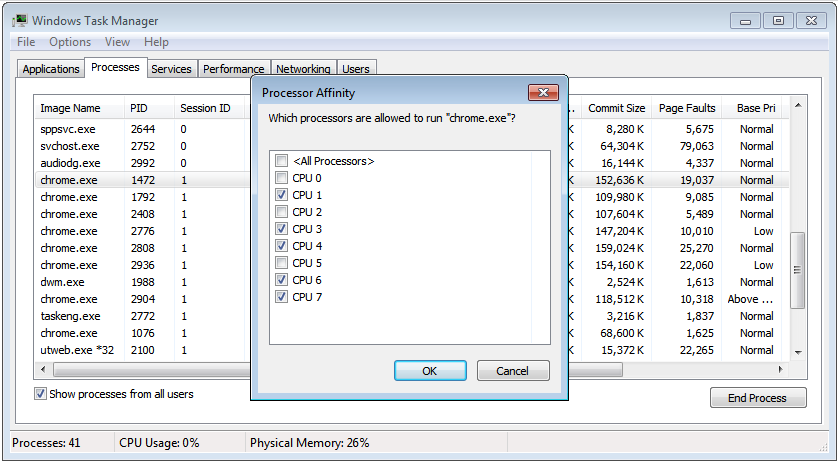
\includegraphics[scale=0.6]{affinity1}
	\end{center}

	\begin{center}
		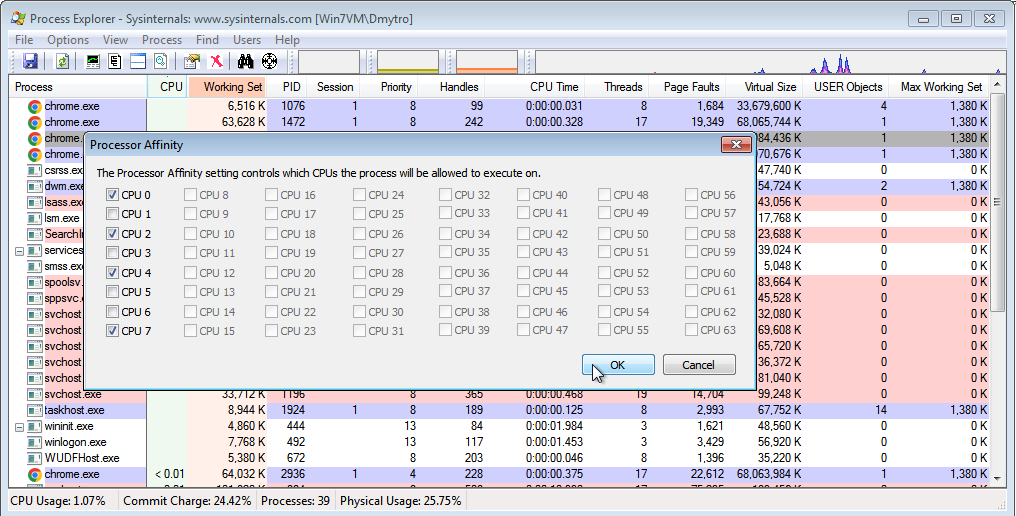
\includegraphics[scale=0.49]{affinity2}
	\end{center}

	\subsection*{3.3 Завершити виконання процесу.}
	\begin{center}
		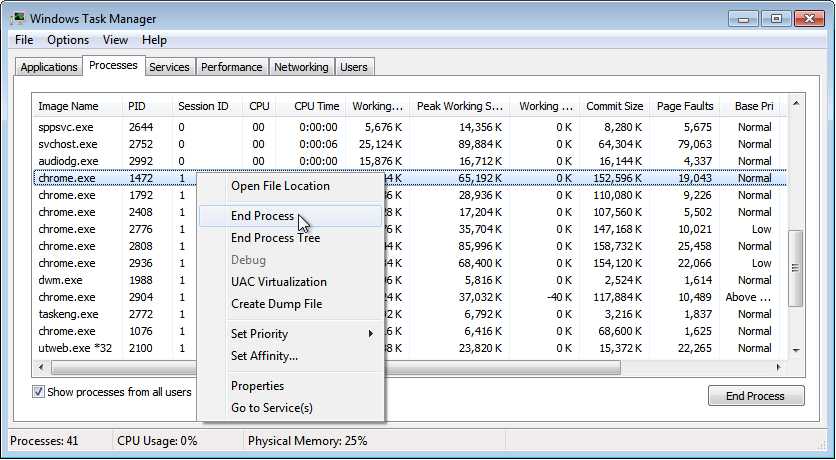
\includegraphics[scale=0.6]{end1}
	\end{center}

	\begin{center}
		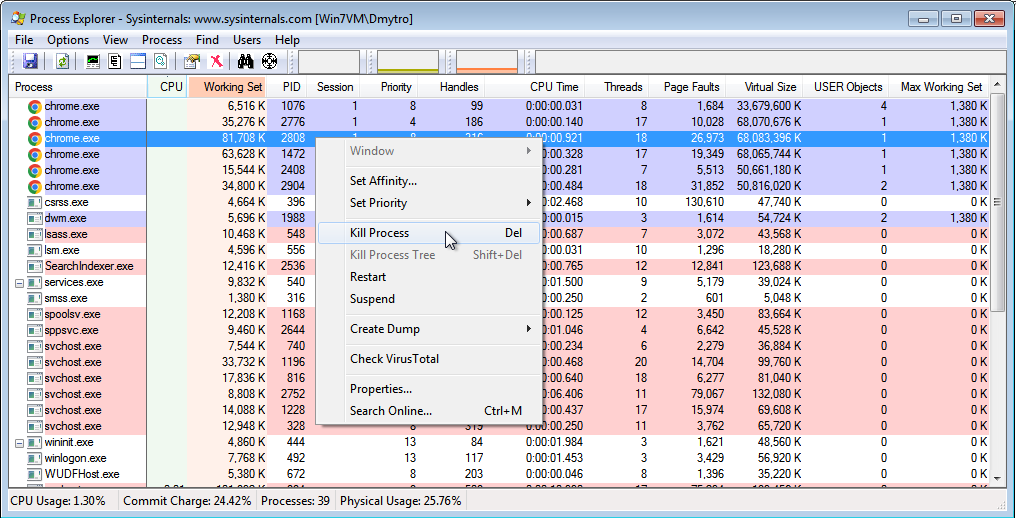
\includegraphics[scale=0.49]{end2}
	\end{center}

	\subsection*{4.1 Призупинити виконання процесу.}
	\begin{center}
		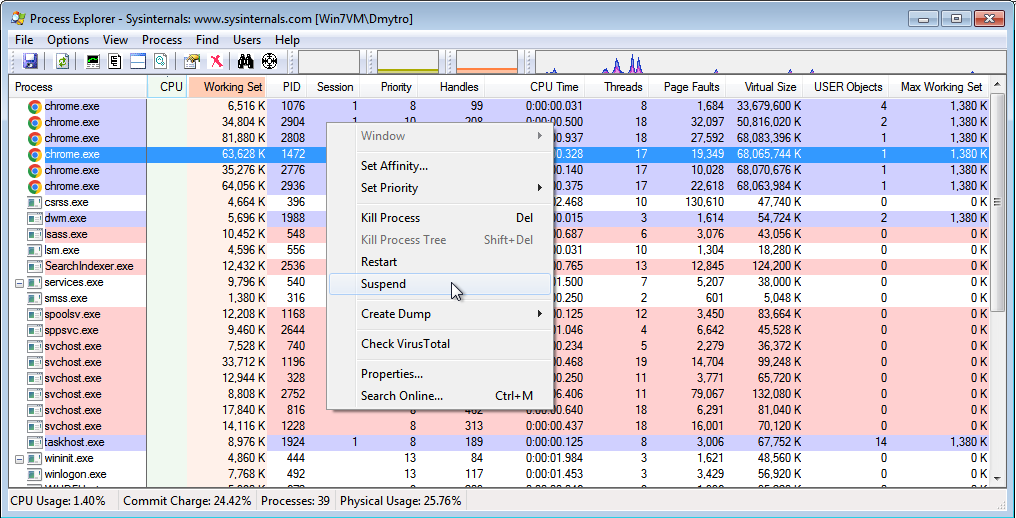
\includegraphics[scale=0.49]{suspend1}
	\end{center}

	\subsection*{4.2 Продовжити виконання процесу.}
	\begin{center}
		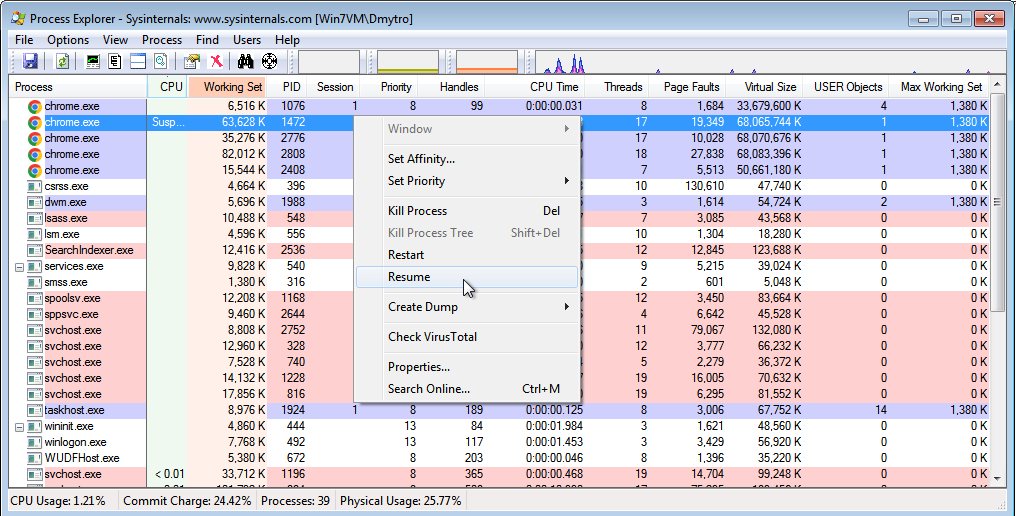
\includegraphics[scale=0.49]{suspend2}
	\end{center}

	\subsection*{5. Визначити A, S, p при різних n для скомпільованої програми.}
	\begin{gather}\nonumber
		n=1; T_1=20\text{мс}; A=S=1; p=p.\\\nonumber
		n=2; T_2 =15\text{мс}; A=S=1.33; p=0.5.\\\nonumber
		n=3; T_3 =14\text{мс}; A=S=1.42; p=0.55.\\\nonumber
		n=4; T_4 =14\text{мс}; A=S=1.42; p=0.6.\\\nonumber
		n=5; T_5 =15\text{мс}; A=S=1.33; p=0.68.\\\nonumber
		n=6; T_6 =14\text{мс}; A=S=1.42; p=0.64.\\\nonumber
		n=7; T_7 =16\text{мс}; A=S=1.25; p=0.76.\\\nonumber
		n=8; T_8 =15\text{мс}; A=S=1.33; p=0.71.\nonumber
	\end{gather}

	\subsection*{6. Дослідити залежність швидкості стискання файлу від кількості доступних ядер ЦП.}
	Я виконав стискання файлу розміром 730Мб за допомогою програми 7-zip, попередньо встановивши за допомогою функції "Set Affinity" кількість ядер процесора \textbf{n}, доступних для програми та отримав результат $\bm{T_n}$, що відповідає часу виконання стискання виміряного в секундах.
	\begin{gather}\nonumber
		n=1; T_1=28c.\\\nonumber
		n=2; T_2=8c.\\\nonumber
		n=3; T_3=8c.\\\nonumber
		n=4; T_4=5c.\\\nonumber
		n=5; T_5=5c.\\\nonumber
		n=6; T_6=4c.\\\nonumber
		n=7; T_7=4c.\\\nonumber
		n=8; T_8=3c.\nonumber
	\end{gather}

	\section*{Висновок}
	Під час виконання лабораторної роботи я за допомогою утиліт "Task Manager" та "Process Explorer" операційної системи Windows отримав повну інформацію про процеси. Використовуючи ці утиліти я змінив пріоритет процесів на пріорітет "Realtime". Задав відповідність процесів на окремих ядрах центрального процесора та завершив виконання процесу. Визначив залежність швидкодії скомпрограми від кількості доступних ядер процесора.
	    
\end{normalsize}
\end{document}
